\section{Introducción}

En esta práctica se pide crear un modelo sencillo y construir un \textit{rig} que permita controlar la animación.

\bigskip

En mi caso, he decidido crear una excavadora que puede girar sobre su propio eje.

\begin{figure}[H]
   \centering
   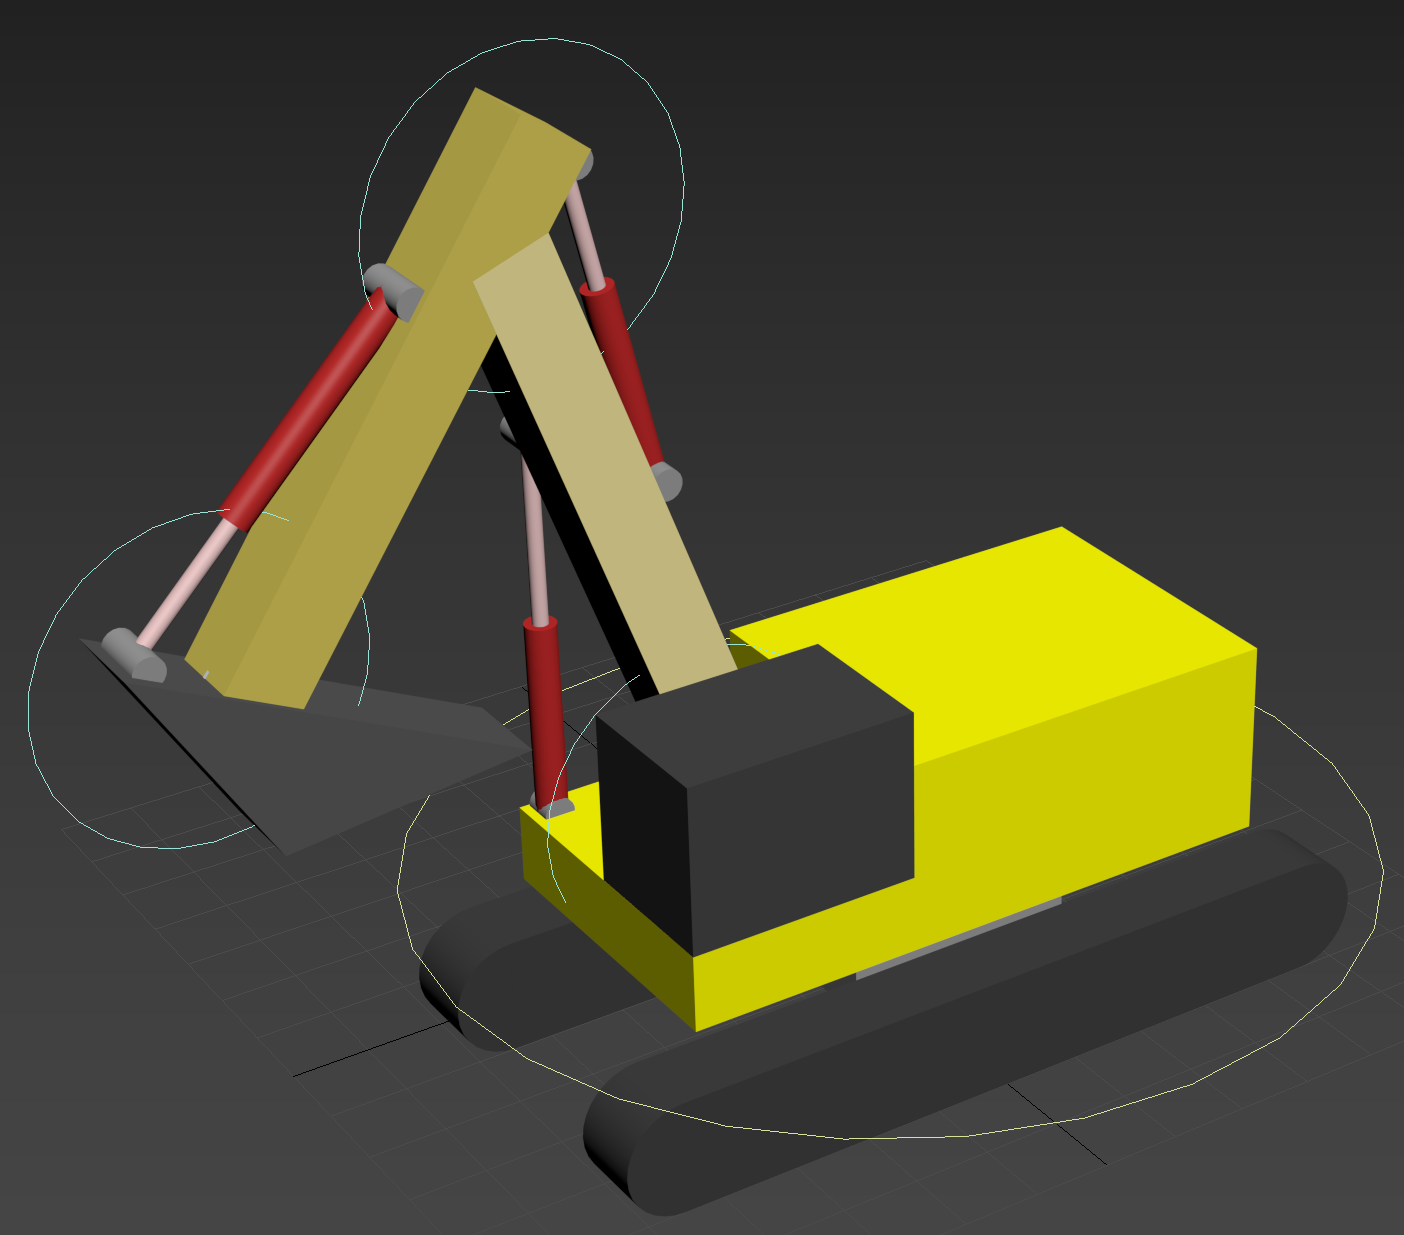
\includegraphics[width=0.5\textwidth]{imagenes/excavadora.png}
   \caption{Modelo final de la excavadora.}
\end{figure}

En las siguientes secciones explicaré el proceso de creación del modelo: